\documentclass[tikz,border=5pt]{standalone}
\usepackage[utf8]{inputenc}
\usepackage[T1]{fontenc}
\usepackage{lmodern,amsmath,amssymb}
\usepackage[american]{circuitikz}
\usepackage{pgfplots}
\pgfplotsset{compat=1.18}
\usetikzlibrary{circuits.logic.US,positioning,calc,arrows.meta,patterns,shapes.geometric}
\definecolor{Primary}{HTML}{1F77B4}
\begin{document}
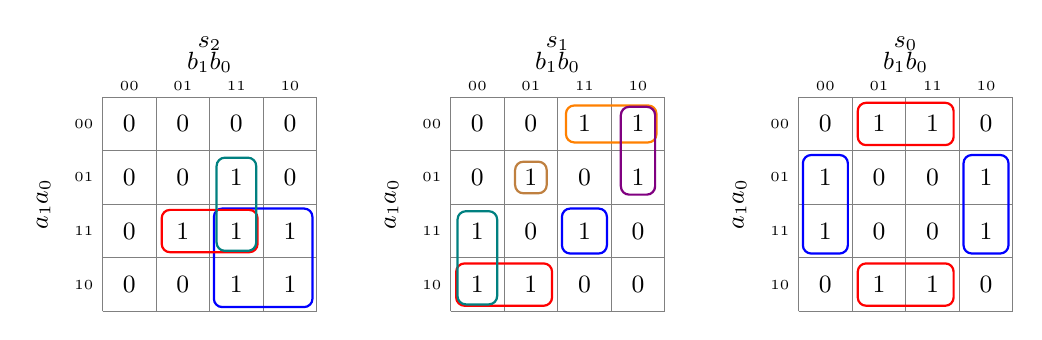
\begin{tikzpicture}[x=.68cm,y=.68cm,font=\small]
\begin{scope}[xshift=0.0cm]
\foreach \k in {0,...,4}{\draw[gray] (\k,0)--(\k,4) (0,\k)--(4,\k);}
\node at (2,5){$s_2$};
\node at (2,4.65){$b_1b_0$};\node[rotate=90] at (-1.1,2){$a_1a_0$};
\node at (0.5,4.2){\tiny 00};\node at (-.35,3.5){\tiny 00};
\node at (1.5,4.2){\tiny 01};\node at (-.35,2.5){\tiny 01};
\node at (2.5,4.2){\tiny 11};\node at (-.35,1.5){\tiny 11};
\node at (3.5,4.2){\tiny 10};\node at (-.35,0.5){\tiny 10};
\node at (0.5,3.5){0};
\node at (1.5,3.5){0};
\node at (2.5,3.5){0};
\node at (3.5,3.5){0};
\node at (0.5,2.5){0};
\node at (1.5,2.5){0};
\node at (2.5,2.5){1};
\node at (3.5,2.5){0};
\node at (0.5,1.5){0};
\node at (1.5,1.5){1};
\node at (2.5,1.5){1};
\node at (3.5,1.5){1};
\node at (0.5,0.5){0};
\node at (1.5,0.5){0};
\node at (2.5,0.5){1};
\node at (3.5,0.5){1};
\draw[blue,rounded corners=3pt,thick] (2.08,0.08) rectangle (3.92,1.92);
\draw[red,rounded corners=3pt,thick] (1.105,1.105) rectangle (2.895,1.895);
\draw[teal,rounded corners=3pt,thick] (2.13,1.13) rectangle (2.87,2.87);
\end{scope}
\begin{scope}[xshift=4.42cm]
\foreach \k in {0,...,4}{\draw[gray] (\k,0)--(\k,4) (0,\k)--(4,\k);}
\node at (2,5){$s_1$};
\node at (2,4.65){$b_1b_0$};\node[rotate=90] at (-1.1,2){$a_1a_0$};
\node at (0.5,4.2){\tiny 00};\node at (-.35,3.5){\tiny 00};
\node at (1.5,4.2){\tiny 01};\node at (-.35,2.5){\tiny 01};
\node at (2.5,4.2){\tiny 11};\node at (-.35,1.5){\tiny 11};
\node at (3.5,4.2){\tiny 10};\node at (-.35,0.5){\tiny 10};
\node at (0.5,3.5){0};
\node at (1.5,3.5){0};
\node at (2.5,3.5){1};
\node at (3.5,3.5){1};
\node at (0.5,2.5){0};
\node at (1.5,2.5){1};
\node at (2.5,2.5){0};
\node at (3.5,2.5){1};
\node at (0.5,1.5){1};
\node at (1.5,1.5){0};
\node at (2.5,1.5){1};
\node at (3.5,1.5){0};
\node at (0.5,0.5){1};
\node at (1.5,0.5){1};
\node at (2.5,0.5){0};
\node at (3.5,0.5){0};
\draw[blue,rounded corners=3pt,thick] (2.08,1.08) rectangle (2.92,1.92);
\draw[red,rounded corners=3pt,thick] (0.10500000000000001,0.10500000000000001) rectangle (1.895,0.895);
\draw[teal,rounded corners=3pt,thick] (0.13,0.13) rectangle (0.87,1.87);
\draw[orange,rounded corners=3pt,thick] (2.1550000000000002,3.1550000000000002) rectangle (3.8449999999999998,3.8449999999999998);
\draw[violet,rounded corners=3pt,thick] (3.18,2.18) rectangle (3.82,3.82);
\draw[brown,rounded corners=3pt,thick] (1.205,2.205) rectangle (1.795,2.795);
\end{scope}
\begin{scope}[xshift=8.84cm]
\foreach \k in {0,...,4}{\draw[gray] (\k,0)--(\k,4) (0,\k)--(4,\k);}
\node at (2,5){$s_0$};
\node at (2,4.65){$b_1b_0$};\node[rotate=90] at (-1.1,2){$a_1a_0$};
\node at (0.5,4.2){\tiny 00};\node at (-.35,3.5){\tiny 00};
\node at (1.5,4.2){\tiny 01};\node at (-.35,2.5){\tiny 01};
\node at (2.5,4.2){\tiny 11};\node at (-.35,1.5){\tiny 11};
\node at (3.5,4.2){\tiny 10};\node at (-.35,0.5){\tiny 10};
\node at (0.5,3.5){0};
\node at (1.5,3.5){1};
\node at (2.5,3.5){1};
\node at (3.5,3.5){0};
\node at (0.5,2.5){1};
\node at (1.5,2.5){0};
\node at (2.5,2.5){0};
\node at (3.5,2.5){1};
\node at (0.5,1.5){1};
\node at (1.5,1.5){0};
\node at (2.5,1.5){0};
\node at (3.5,1.5){1};
\node at (0.5,0.5){0};
\node at (1.5,0.5){1};
\node at (2.5,0.5){1};
\node at (3.5,0.5){0};
\draw[blue,rounded corners=3pt,thick] (0.08,1.08) rectangle (0.92,2.92);
\draw[blue,rounded corners=3pt,thick] (3.08,1.08) rectangle (3.92,2.92);
\draw[red,rounded corners=3pt,thick] (1.105,3.105) rectangle (2.895,3.895);
\draw[red,rounded corners=3pt,thick] (1.105,0.10500000000000001) rectangle (2.895,0.895);
\end{scope}
\end{tikzpicture}
\end{document}
